\pdfminorversion=4

\documentclass{beamer}

\usepackage[T1]{ fontenc }
\usepackage[utf8]{ inputenc }
\usepackage{ drawstack }
\usepackage{ lmodern }
\usepackage{ color }
\usepackage{ graphicx }
\graphicspath{ {./pix/} }

\usetheme{metropolis}

\title{Basic pwning with r2.}
\date{\today}
\author[jvoisin]{Julien (jvoisin) Voisin}
\institute{r2con}

\begin{document}

\maketitle

\begin{frame}{whoami}
    \begin{center}
        \Large Julien (jvoisin) Voisin\\dustri.org
    \end{center}
\end{frame}

\begin{frame}{Quizz}
    \begin{itemize}[<+->]
        \item ASLR/PIE/NX/Canary
        \item GOT/PLT
        \item mona.py/peda
        \item CTF
        \item Heap feng shui
    \end{itemize}
\end{frame}

% Put the clever people on io and overthewire
\begin{frame}{1337-hackerz}
	Radare2 is available on \alert{io}\footnote{http://io.smashthestack.org/}
	and \alert{overthewire}\footnote{http://overthewire.org/wargames/}.

	\begin{center}
		\pause So \emph{take off your hats and go corrupt some memor-y-ies}.
	\end{center}
\end{frame}


\section{Crash course}
\begin{frame}{Exploitation}
	\begin{block}{Exploitation}
		An exploit is a piece of software [\dots] that takes advantage of [\dots] vulnerability in order to [\dots] gain control of a computer system.
	\end{block}
	\begin{center}
		This workshop is about memory corruption.
	\end{center}
\end{frame}

% Show what is a program
\begin{frame}{Our playground}
	\begin{center}
		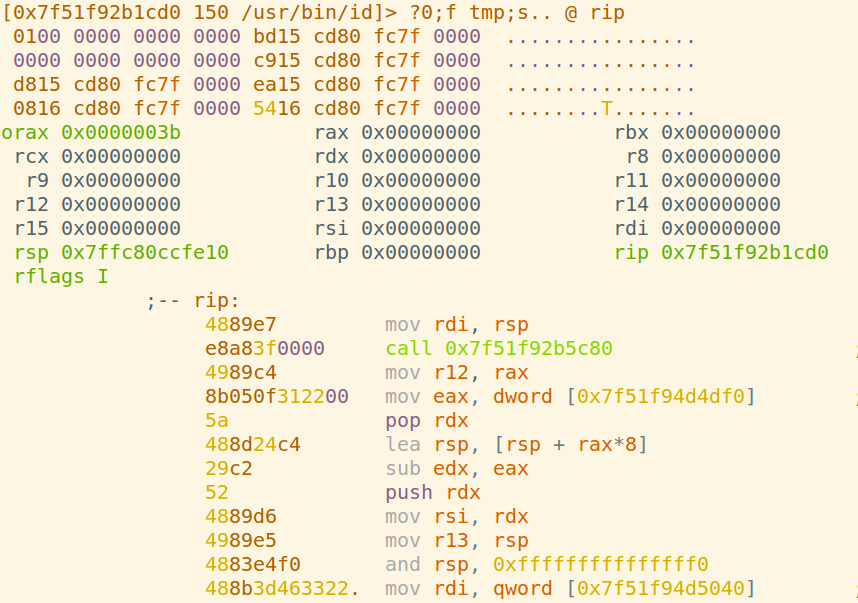
\includegraphics[height=6.5cm,width=\textwidth,trim = 0mm 12cm 0mm 0mm, clip]{regstacklisting.png}
	\end{center}
\end{frame}

% What is a stack
\begin{frame}{Stack}
	\begin{center}
	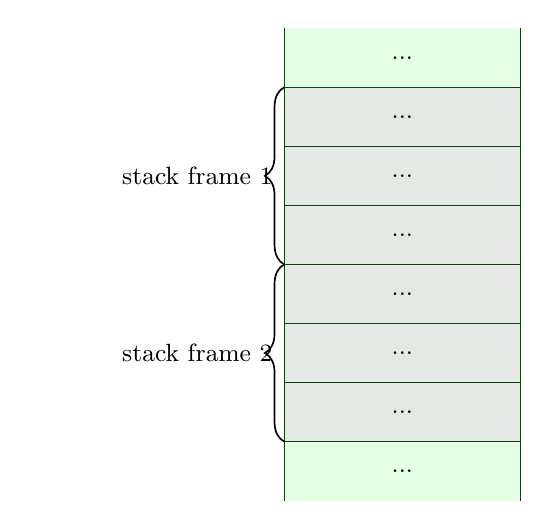
\begin{tikzpicture}[scale=0.75]
		\small
		\stacktop{}
		\startframe
		\padding{1}{...}
		\padding{1}{...}
		\padding{1}{...}
		\finishframe{stack frame 1}
		\startframe
		\padding{1}{...}
		\padding{1}{...}
		\padding{1}{...}
		\finishframe{stack frame 2}
		\stackbottom{}
	\end{tikzpicture}
	\end{center}
\end{frame}

% Mention Aleph One
\begin{frame}{Stack smashing}
	\begin{center}
		\begin{columns}
			\begin{column}{.5\textwidth}
				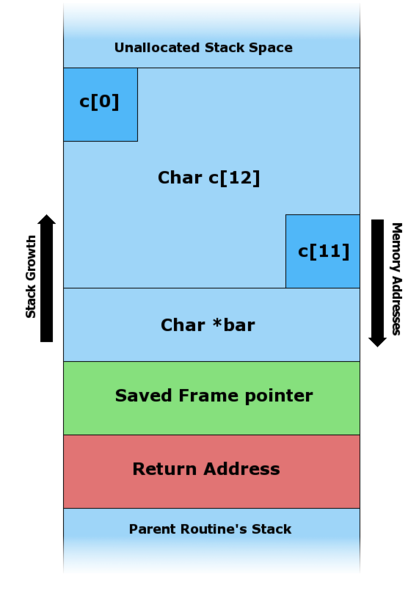
\includegraphics[height=6.5cm]{overflow1.png}
			\end{column}
			\begin{column}{.5\textwidth}
				\only<1>{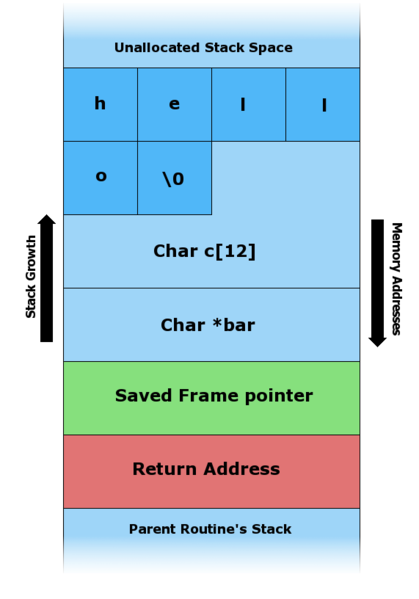
\includegraphics[height=6.5cm]{overflow2.png}}
				\only<2>{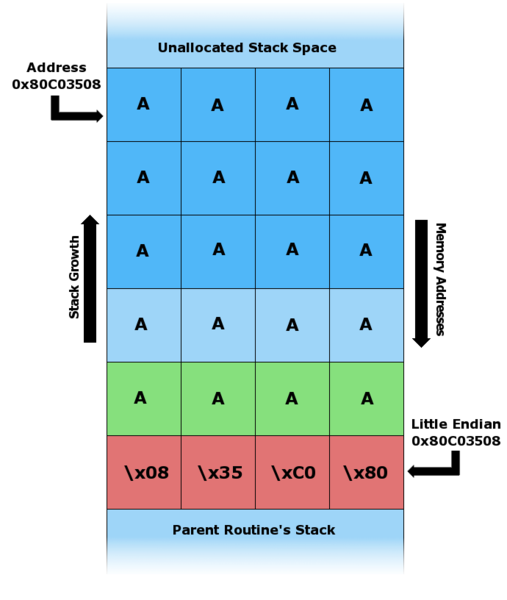
\includegraphics[height=6.5cm]{overflow3.png}}
			\end{column}
		\end{columns}
	\end{center}
\end{frame}

% This is needed later for system-wide ASLR bypass
\begin{frame}{ASLR and GOT}
	\begin{center}
	\only<1>{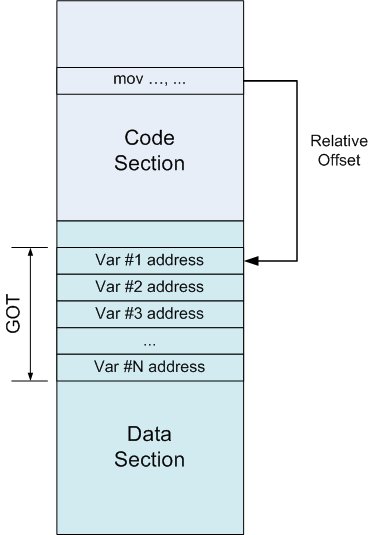
\includegraphics[height=6cm]{got.png}}
	\only<2>{
		\begin{columns}
			\begin{column}{.5\textwidth}
				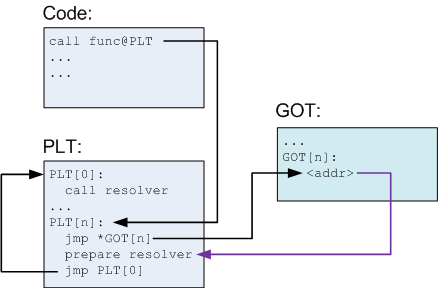
\includegraphics[width=\textwidth]{plt_before.png}
			\end{column}
			\begin{column}{.5\textwidth}
				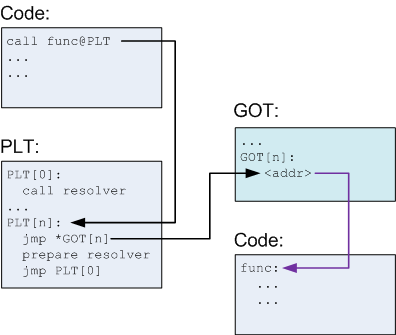
\includegraphics[width=\textwidth]{plt_after.png}
			\end{column}
		\end{columns}
	}
	\end{center}
\end{frame}

\section{Disclaimer}
\begin{frame}{Disclaimer}
    \begin{itemize}
        \item The challenges are from old CTF
        \item So you'll be able to reproduce other writeups
        \item Don't cheat, cheating is bad, m'kay.
    \end{itemize}
\end{frame}

\section{r0pbaby}
\begin{frame}{r0pbaby}
    \begin{itemize}
        \item Defcon CTF Quals 2015
        \item \emph{easy}
        \item x64, NX, PIE and ASLR
    \end{itemize}
\end{frame}

\begin{frame}{Leak}
    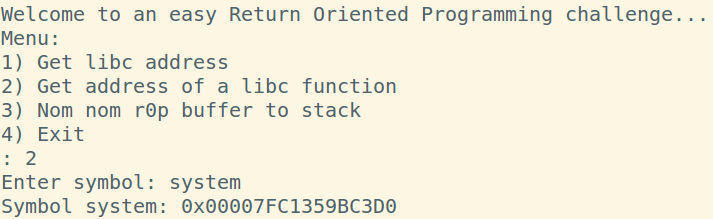
\includegraphics[width=\textwidth]{r0pbaby_leak.png}
\end{frame}

\begin{frame}{Your turn}
    \begin{center}
        \Large Get a crash
    \end{center}
\end{frame}

\begin{frame}{Crash}
    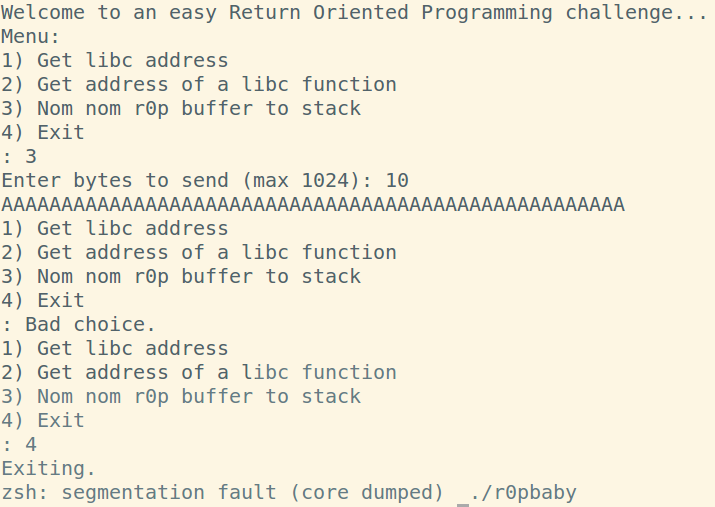
\includegraphics[width=\textwidth]{r0pbaby_crash.png}
\end{frame}

\begin{frame}{Control of RIP}
    \begin{semiverbatim}
    r2 -b64 -d rarun2 program="r0pbaby"

    input="3\\n10\\nAAAAAAAAAAAAAAAAAAAAAAAAAAAA\\n4\\n"

    stdout=/dev/null
\end{semiverbatim}
\end{frame}

\begin{frame}{Control of RIP}
    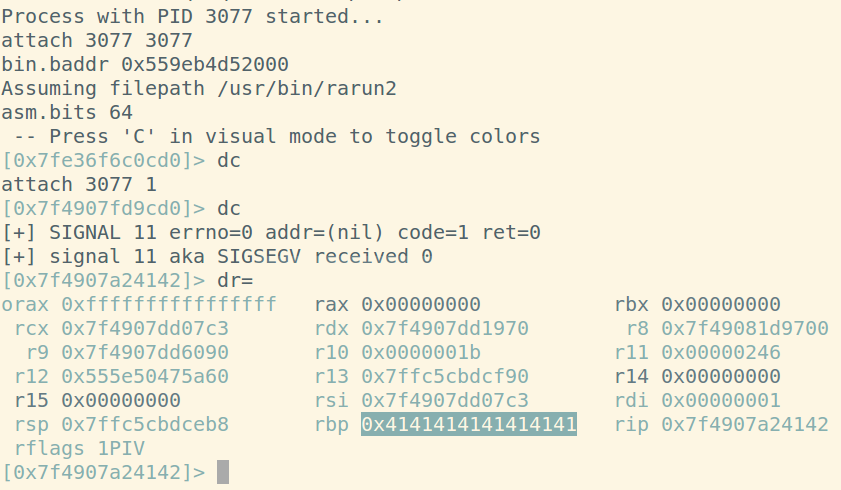
\includegraphics[width=\textwidth]{r0pbaby_r2d.png}
\end{frame}

\begin{frame}{Your turn}
    \begin{center}
        \Large Get control of RIP
    \end{center}
\end{frame}

\begin{frame}{Control of RIP}
    \begin{semiverbatim}
    r2 -b64 -d rarun2 program="r0pbaby"

    input="3\\n10\\nAAAAAAAAAAAAAAAAAAAAAAAAAAAA\\n4\\n"

    stdout=/dev/null
\end{semiverbatim}
\end{frame}

\begin{frame}{Finding the right offset}
    \begin{semiverbatim}
    r2 -b64 -d rarun2 program="r0pbaby"

    input="3\\n12\\nAAAAAAAABBBBBBBB\\n4\\n" stdout=/dev/null
\end{semiverbatim}
\end{frame}

\begin{frame}{Finding the right offset}
    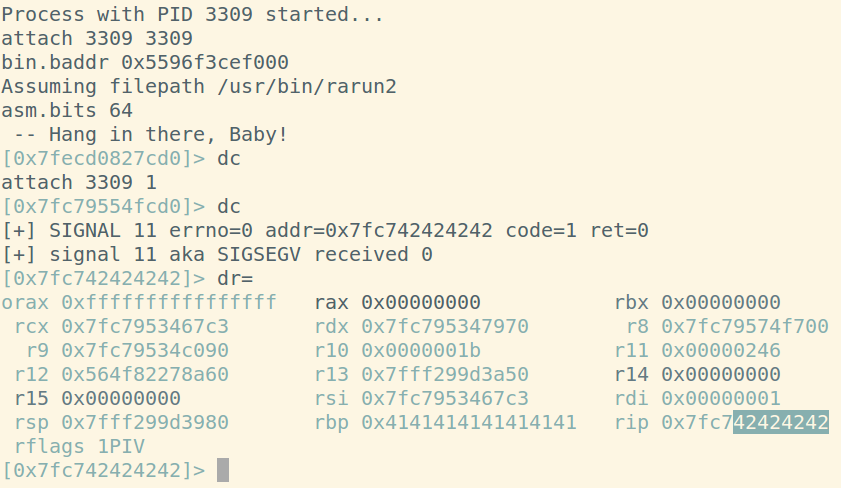
\includegraphics[width=\textwidth]{r0pbaby_rip.png}
\end{frame}

\begin{frame}{Exploit?}
        \begin{center}
            Put the shellcode into an \emph{env} variable and then jump on it?
    \vskip2em
    \only<2>{
            \alert{Nope:} ASLR et NX
    }
        \end{center}
\end{frame}

\begin{frame}{ROP saves the party!}
    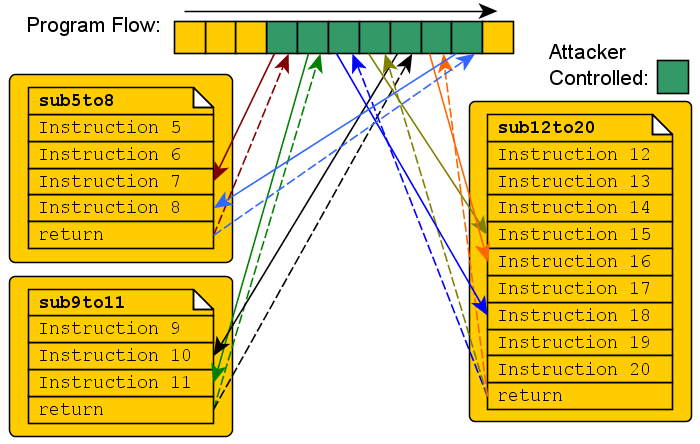
\includegraphics[width=\textwidth]{rop.png}
\end{frame}

\begin{frame}{Calling convention}
    \begin{block}{x86}
        \begin{itemize}
            \item Arguments on the stack
            \item pop-ret
        \end{itemize}
    \end{block}
    \begin{block}{x86-64}
        \begin{itemize}
            \item Arguments in registerrs
            \item pop rdi-ret, pop rsi-ret, \dots
        \end{itemize}
    \end{block}
\end{frame}

\begin{frame}{Attack plan}
    \begin{enumerate}
        \item Getting the address of \alert{system}
        \item Computing the constant offset between
            \begin{enumerate}
                \item \alert{/bin/sh} and \alert{system}
                \item a \alert{pop rdi-ret} gadget and \alert{system}
            \end{enumerate}
        \item Push on the stack
            \begin{enumerate}
                \item Our \alert{gadget}
                \item The offset of \alert{/bin/sh}
                \item The offset of \alert{system}
            \end{enumerate}
        \item Trigger the vulnerability
    \end{enumerate}
\end{frame}

\begin{frame}{Our ROP-chain}
    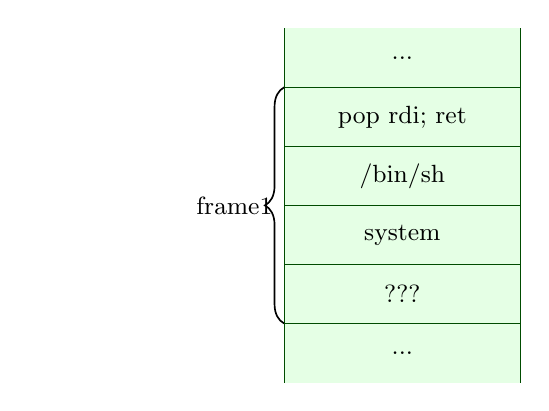
\begin{tikzpicture}[scale=0.75]
        \small
        \stacktop{}
        \startframe
        \cell{pop rdi; ret}
        \cell{/bin/sh}
        \cell{system}
        \cell{???}
        \finishframe{frame1}
        \stackbottom{}
    \end{tikzpicture}
\end{frame}


\begin{frame}{Libc}
    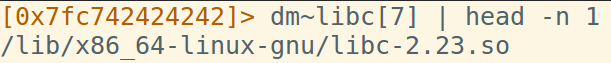
\includegraphics[width=\textwidth]{r0pbaby_dm.png}
    \begin{itemize}
        \item \alert{dm} stands for \alert{d}ebug \alert{m}aps
        \item \alert{$\tilde{}$ $[7]$} to select the $7^{th}$ column
        \item \alert{|} to pipe r2's output
    \end{itemize}
\end{frame}

\begin{frame}{Your turn}
    \begin{center}
        \Large
        \begin{itemize}
            \item Get the offset of the \alert{system} \emph{s}ymbol
            \item Get the offset of the \alert{/bin/sh} \emph{s}tring\footnote{Pronounce it with a German accent.}
            \item Compute the difference between them
        \end{itemize}
    \end{center}
\end{frame}

\begin{frame}{/bin/sh}
    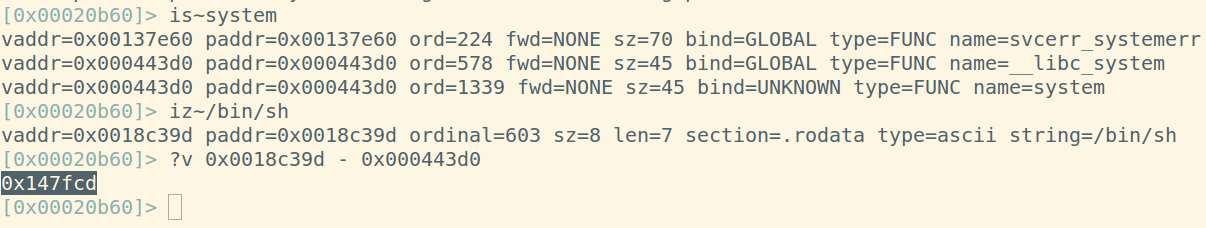
\includegraphics[width=1.1\textwidth]{r0pbaby_binsh.png}
\end{frame}

\begin{frame}{popret!}
    \begin{center}
        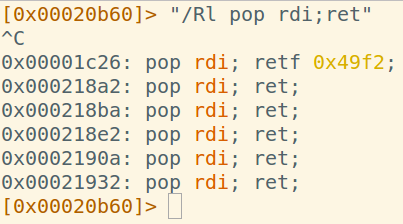
\includegraphics[width=.7\textwidth]{r0pbaby_popret.png}
    \end{center}
    \begin{center}
        Protip: \alert{e search.<tab>}
    \end{center}
\end{frame}

\begin{frame}{Our ROP-chain}
    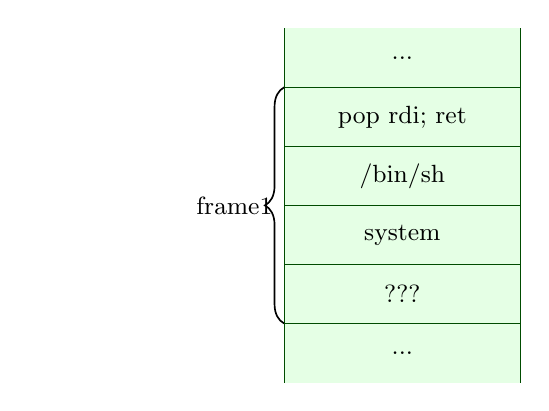
\begin{tikzpicture}[scale=0.75]
        \small
        \stacktop{}
        \startframe
        \cell{pop rdi; ret}
        \cell{/bin/sh}
        \cell{system}
        \cell{???}
        \finishframe{frame1}
        \stackbottom{}
    \end{tikzpicture}
\end{frame}

\begin{frame}{Your turn}
    \begin{center}
        \Large Get a shell!
    \end{center}
    \begin{itemize}
        \item \alert{/R}  -- Rop-search
        \item \alert{iz}  -- strings\footnote{Still with the German accent}
        \item \alert{is}  -- symbols
    \end{itemize}
\end{frame}

\begin{frame}{Demo}
    \begin{center}
        \Large Demo!
    \end{center}
\end{frame}


\section{exp400 of the Nullcon 2014}
\begin{frame}{exp400 de la Nullcon 2014}
    \begin{itemize}
        \item Nullcon - A neat conference in India
        \item With a cool CTF
        \item A not-so-tricky challenge: no PIE, no canary.
    \end{itemize}
\end{frame}

\begin{frame}{Your turn}
    \begin{center}
        \Large Find what this binary is doing
    \end{center}
\end{frame}

\begin{frame}{Long story short...}
    The binary is:
    \begin{enumerate}
        \item Allocating some memory on the heap
        \item Opening the \alert{flag} file
        \item Dropping its permissions
        \item Writing the content of the file on the allocated space ("the\_amazing\_pancake" in our case)
        \item Closing the \emph{file descriptor}
        \item Writing a message to the user
        \item Write a user-controlled input into the heap
    \end{enumerate}
    We need to walk the heap!
\end{frame}

\begin{frame}{ASLR}
    \begin{center}
    The stack is subject to ASLR, and the heap too.\\

    Fortunately, it's \alert{deterministic}.
    \end{center}
\end{frame}

\begin{frame}{Steps}
    \begin{enumerate}
        \item Get a crash
        \item Get control of EIP
        \item Find a leak to defeat ASLR
        \item Build a ROP-chain
        \item Perform a small victory dance
    \end{enumerate}
\end{frame}

\begin{frame}{De Bruijn}
    \begin{center}
        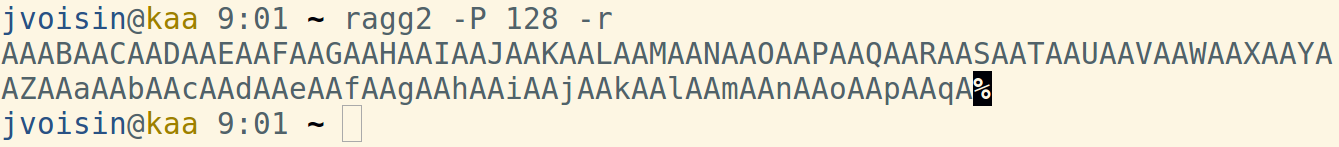
\includegraphics[width=\textwidth]{debruijn.png}
        \begin{itemize}
            \item A cyclic sequence in which every sequences of a given size,
                of a given alphabet are occurring exactly once
            \item Handy to find the right padding
        \end{itemize}
    \end{center}
\end{frame}

\begin{frame}{Offset}
    \begin{center}
        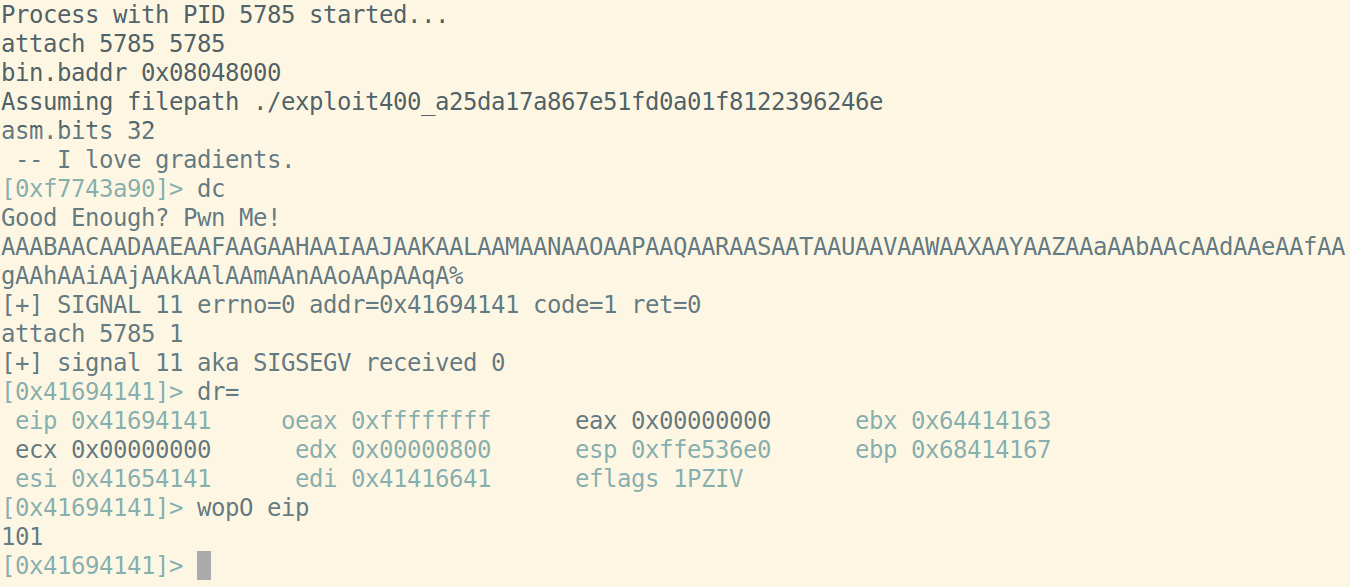
\includegraphics[width=\textwidth]{exploit400_eip.png}
    \end{center}
\end{frame}

\begin{frame}{How to get the flag?}
    \begin{itemize}
        \item The binary is x86 and non-PIE
        \item We have a code-execution
        \item Heap is deterministic
        \item Lets call \alert{malloc} to get the right offset into \alert{eax}
        \item Add the right padding to get the offset of the flag, relatively to \alert{eax}'s value
        \item Call \alert{write} on this offset
    \end{itemize}
\end{frame}

\begin{frame}{Our ROP-chain so far}
    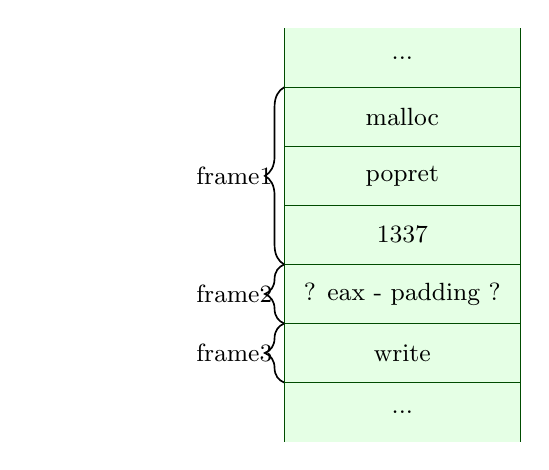
\begin{tikzpicture}[scale=0.75]
        \small
        \stacktop{}
        \startframe
        \cell{malloc}
        \cell{popret}
        \cell{1337}
        \finishframe{frame1}
        \startframe
        \cell{? eax - padding ?}
        \finishframe{frame2}
        \startframe
        \cell{write}
        \finishframe{frame3}
        \stackbottom{}
    \end{tikzpicture}
\end{frame}

\begin{frame}{How to get the flag}
    \begin{center}
        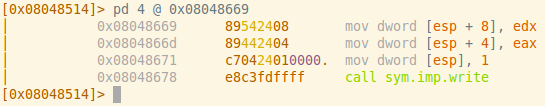
\includegraphics[width=\textwidth]{exp400_write.png}
        \begin{itemize}
            \item \alert{edx}: size of the string
            \item \alert{eax}: pointer to the string
            \item \alert{1}: file descriptor
        \end{itemize}
    \end{center}
\end{frame}

\begin{frame}{Strlen}
    \begin{center}
        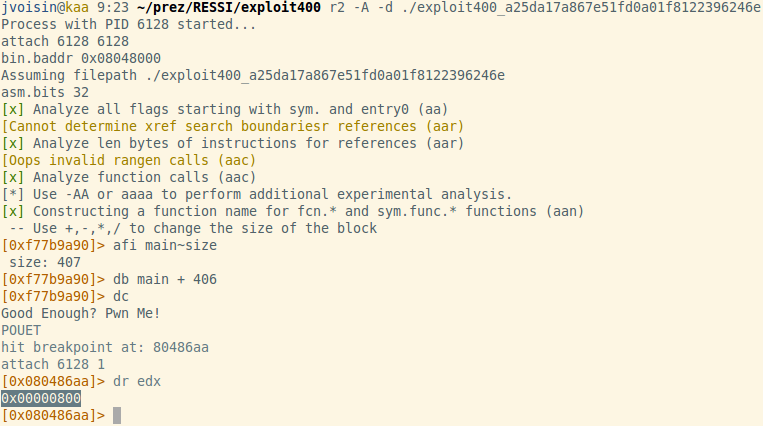
\includegraphics[width=\textwidth]{exp400_edx.png}
    \end{center}
\end{frame}

\begin{frame}{Your turn}
    \begin{center}
        \Large
        \begin{itemize}
            \item Find the offset of \alert{malloc}
            \item Find a \alert{pop-ret} gadget
        \end{itemize}
    \end{center}
\end{frame}

\begin{frame}{Calling malloc}
    \begin{center}
            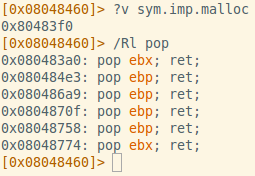
\includegraphics[width=.7\textwidth]{exp400_imp.png}
    \end{center}
\end{frame}

\begin{frame}{Offset between our \alert{malloc} and the flag}
    \begin{center}
        \only<1>{
            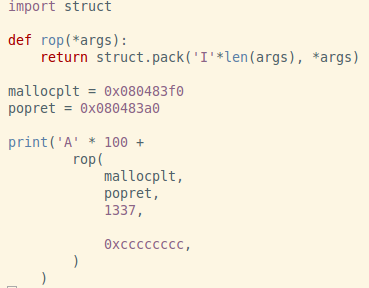
\includegraphics[width=.75\textwidth]{exp400_get_offset.png}
        }
        \only<2>{
            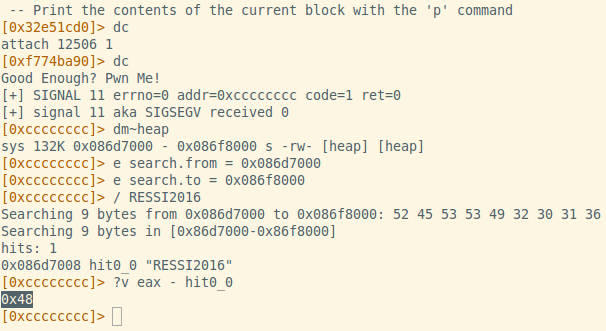
\includegraphics[width=\textwidth]{exp400_malloc_offset.png}
        }
    \end{center}
\end{frame}

\begin{frame}{Subtraction of the right offset}
    \only<1>{
    We could:
    \begin{itemize}
        \item Call \alert{malloc} to get the offset
        \item Call \alert{write} to send it back to us
        \item Subtract \alert{0x48}
        \item Call \alert{read} to read the result somewhere
        \item Use this result in a \alert{write} to get the flag
    \end{itemize}
}
\only<2>{
    But instead, we're going to:
    \begin{itemize}
        \item Call \alert{malloc} to get the offset
        \item Subtract \alert{0x48} with a gadget
        \item Use this result in a \alert{write} to get the flag
    \end{itemize}
}
\end{frame}

\begin{frame}{Our ROP-chain}
    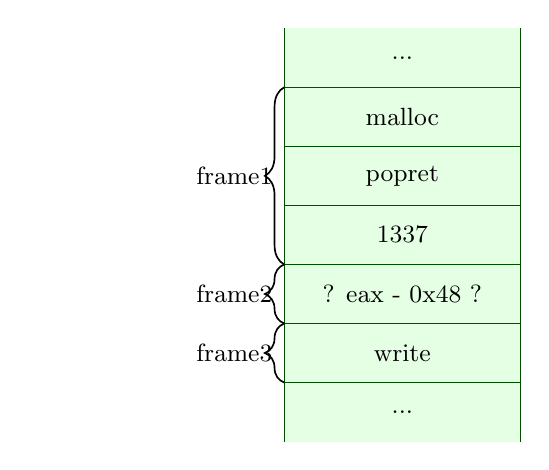
\begin{tikzpicture}[scale=0.75]
        \small
        \stacktop{}
        \startframe
        \cell{malloc}
        \cell{popret}
        \cell{1337}
        \finishframe{frame1}
        \startframe
        \cell{? eax - 0x48 ?}
        \finishframe{frame2}
        \startframe
        \cell{write}
        \finishframe{frame3}
        \stackbottom{}
    \end{tikzpicture}
\end{frame}

\begin{frame}{Subtraction of 0x48}
    \begin{center}
            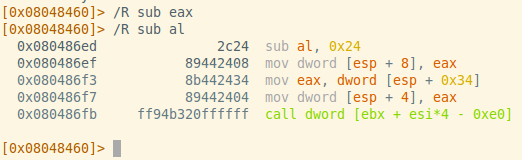
\includegraphics[width=\textwidth]{exp400_gadgets.png}\\
            Ouch.
    \end{center}
\end{frame}

\begin{frame}{Your turn}
    \begin{center}
        \Large Find a gadget to \alert{sub 0x48}\footnote{check \alert{libr/asm/d/x86}}
    \end{center}
\end{frame}


\begin{frame}{Subtraction of 0x48}
    \begin{center}
            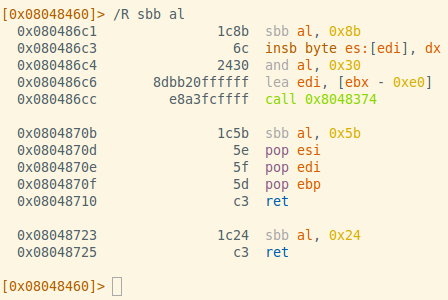
\includegraphics[width=\textwidth]{exp400_sbb.png}
    \end{center}
\end{frame}

\begin{frame}{Our ROP-chain}
    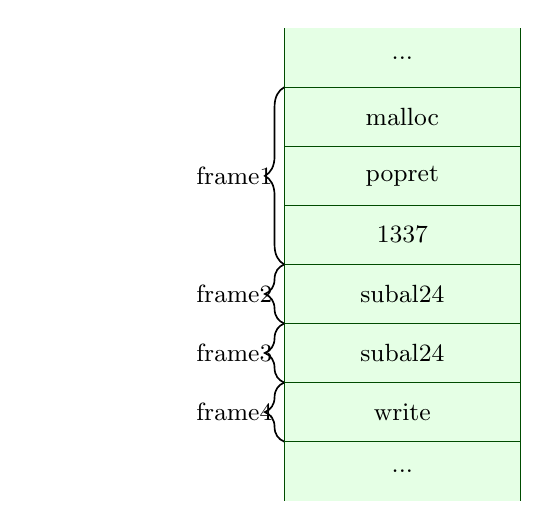
\begin{tikzpicture}[scale=0.75]
        \small
        \stacktop{}
        \startframe
        \cell{malloc}
        \cell{popret}
        \cell{1337}
        \finishframe{frame1}
        \startframe
        \cell{subal24}
        \finishframe{frame2}
        \startframe
        \cell{subal24}
        \finishframe{frame3}
        \startframe
        \cell{write}
        \finishframe{frame4}
        \stackbottom{}
    \end{tikzpicture}
\end{frame}

\begin{frame}{Your turn}
    \begin{center}
        \Large Get the flag!
    \end{center}
\end{frame}

\begin{frame}{Demo}
    \begin{center}
        \Large Demo!
    \end{center}
\end{frame}

\begin{frame}
    \begin{center}
        \Large Questions?
    \end{center}
\end{frame}

\end{document}
